The semeion-digits dataset will be used throughout this report. It consists of 1593 scanned handwritten digits from around 80 persons, stretched in a rectangular $16\times16$ box in a binary scale. These binary images are then \textit{flattened} into 256 dimensional vectors, yielding a dataset with 1593 observations and 256 features.
\begin{figure}[]
	\centering
	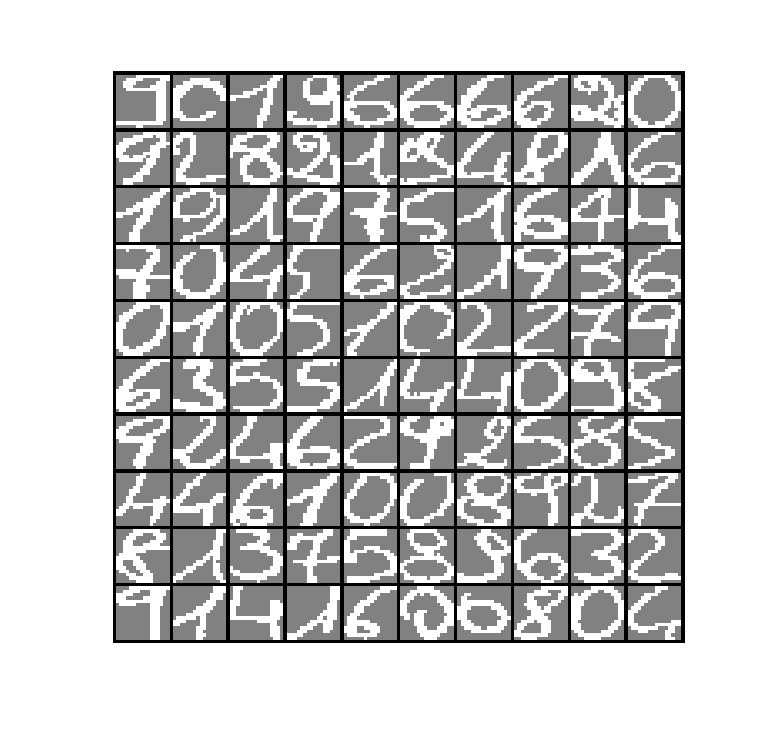
\includegraphics[width=0.4\textwidth, trim={25 25 25 25}, clip]{random_digits}
	\caption{Randomly picked samples of semeion-digits dataset.}
	\label{fig:random_digits}
\end{figure}

The $k$-NN algorithm was implemented in \textsc{Matlab} as a class. The following snippet exemplifies its use.
\begin{lstlisting}
% 50% for training - 50% for testing 
[train, test] = stratified_split(X, t, 0.50);

% create classifier object
k = 10;
kNN = kNNKlassifier(k);

% set hyper-parameters
kNN.distfcn = 'Euclidean';  % (by default) also possible: 'Manhattan'
kNN.weightfcn = 'equal';    % (by default) also possible: 'invdist' or 'rank'

% train classifier
kNN.learn(train.X, train.t);

% get predicted output and compute its accuracy
y_pred = kNN.predict(test.X);
acc = mean( test.t == y_pred );	% accuracy
\end{lstlisting}

The results obtained after executing the previous script can be better visualized with the confusion matrix in figure \ref{fig:confmat_1}. Since there are 10 classes (one per digit) the dimension of the matrix will be $10 \times 10$ whose rows indicate the true label/class, and columns the prediction.
\begin{figure}
	\centering
	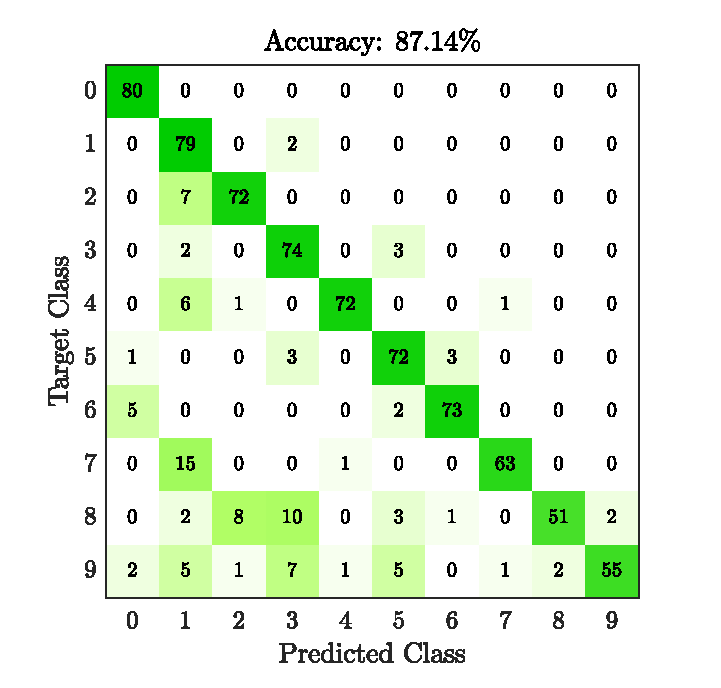
\includegraphics[width=0.4\textwidth]{confmat_1}
	\caption{$k$-NN confusion matrix ($k$ = 10).}
	\label{fig:confmat_1}
\end{figure}

The percentage of samples per class is roughly equal throughout all the semeion dataset, that is, each class takes up around 10\% of the whole dataset. Since we're using stratified split, these percentages are preserved. Sorting out all the evident computations, the test set contains around 80 samples per class. Knowing this can help us get a better grasp of the numbers contained in the confusion matrix in figure \ref{fig:confmat_1}. Moreover, we can see that the most \textit{confused} classes are $1 \gets 7$ and $3 \gets 8$.

Going back to the terminology presented in the introduction, we can say that the diagonal elements are the equivalent of true positives/negatives depending on the class to be analyzed. Additionally, rows represent false negatives and columns represent false positives (omitting diagonal values). Accuracy and misclassification rates are class-independent since they only rely on right or wrong predictions; the remaining class-dependent rates are displayed in table \ref{tbl:rates_1}.
\begin{table}[]
	% increase table row spacing, adjust to taste
	% \renewcommand{\arraystretch}{1.3}
	% if using array.sty, it might be a good idea to tweak the value of
	% \extrarowheight as needed to properly center the text within the cells
	\caption{$k$-NN class-dependent rates}
	\label{tbl:rates_1}
	\centering
	% Some packages, such as MDW tools, offer better commands for making tables
	% than the plain LaTeX2e tabular which is used here.
	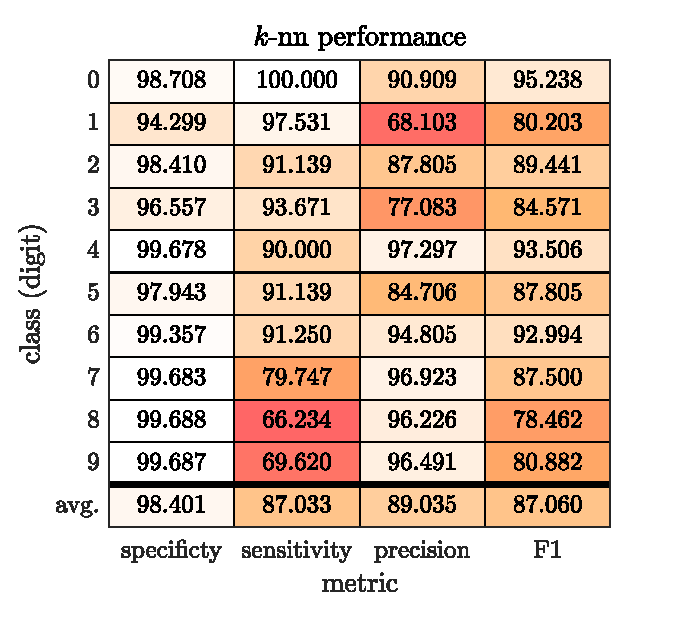
\includegraphics[width=0.4\textwidth]{rates_1}
\end{table}
\begin{figure}
	\centering
	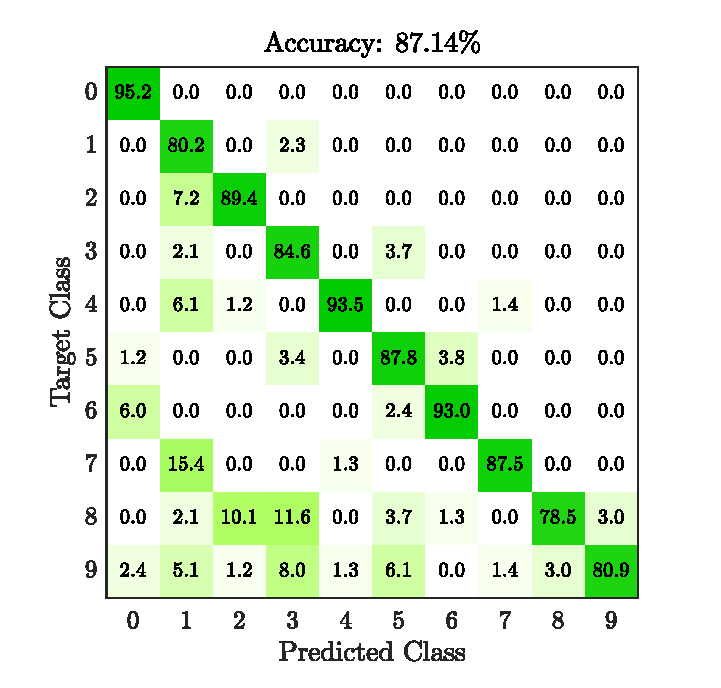
\includegraphics[width=0.4\textwidth]{confmat_2}
	\caption{$k$-NN confusion matrix with F1 scores ($k$ = 10).}
	\label{fig:confmat_2}
\end{figure}

To get a better understanding on the relation between performance rates and the confusion matrix we'll take digit 8 as an example. From table \ref{tbl:rates_1} we notice it has low sensitivity (large number of false negatives, dense row-vector) and high precision (small number of false positives, sparse column-vector). In less technical terms, around 30\% of actual 8 samples get misclassified, but when we predict 8 we can be pretty confident the sample is an actual 8. The F1 score conveys a balance between these two concepts and we will therefore mainly use this score to asses the classifier's performance.

Now, both the confusion matrix and the class-dependent rates provide useful complementary information. The confusion matrix is visually attractive, but numbers in it are hard to understand when not given any context on how it was computed. On the other hand, rates are numerically easy to interpret since they range from 1 to 0 (or 100 to 0) where 1 is the best performance and 0 is worst. Combining them while still retaining the best of both worlds is possible; the \textit{F1-normalized} confusion matrix in figure \ref{fig:confmat_2} is both visually and numerically intuitive.

\subsection{How to choose $k$?}
This is one of the main questions to answer when using $k$-NN. There are multiple approaches to answer this question which, in machine learning, are often referred to as hyper-parameter optimization \cite{hyperparameter-search}. Along with $k$, we have other factors in play such as the distance and weighting functions. Therefore, we'll perform several a \textit{grid search} or \textit{parameter sweep} through a manually specified subset of hyper-parameters.
\begin{gather*}
K \in \left\lbrace 1,2,3,4,5,6,7,8,9,10,12,14,16,18,20 \right\rbrace \\
\texttt{distfcn} \in \left\lbrace \texttt{Euclidean}, \texttt{Manhattan} \right\rbrace \\
\texttt{weightfcn} \in \left\lbrace \texttt{equal}, \texttt{invdist}, \texttt{rank} \right\rbrace
\end{gather*}
%
Regarding the \texttt{distfcn} hyper-parameter, the distance measured by either of the functions is exactly the same since all our features are binary, thus we can discard it from the grid search.
\begin{algorithm}
	\caption{General structure for grid search using a $k$-NN classifier.}
	\label{algo:perceptron}
	\begin{algorithmic}
		\Ensure hyper-parameter subsets initialized
		\Procedure{GridSearch}{\texttt{weightfcn}, $K$, \texttt{iters}}
		\ForAll{$w \in$ \texttt{weightfcn}}
			\ForAll{$k \in K$}
				\For{$i = 1$; $i \leq$ \texttt{iters}; $i$++}
				\State Random train-test split
				\State Train $k$NNClassifier($k, w$) 
				\State Test $k$NNClassifier($k, w$)
				\State Get and store performance metrics
				\EndFor
			\EndFor
		\EndFor
		\EndProcedure		
	\end{algorithmic}
\end{algorithm} 

Binarizing the confusion matrix induces class imbalance, leadint to a positive-negative ratio of 1:9 approximately. Hence, we can avoid displaying true negative rates since they won't greatly contribute to the performance analysis. Figure \ref{fig:knn_rates_2} shows the performance average rates obtained from grid search. It is interesting to note that the shape is mostly preserved among all different metrics due to the stratified splitting. Also, even though the F1 score is considered a balance between precision and recall, this property doesn't hold when averaging though all classes (can also be noted from table \ref{tbl:rates_1}).
\begin{figure}[]
	\centering
	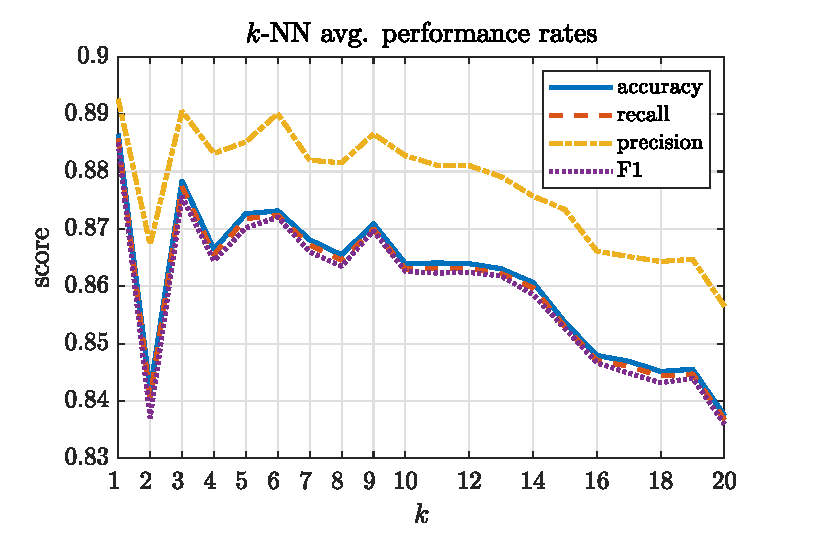
\includegraphics[width=0.45\textwidth]{knn_rates_2}
	\caption{Grid search performance using \texttt{weightfcn} = \texttt{'equal'}. Overall, predictions contain slightly less false positives than false negatives.}
	\label{fig:knn_rates_2}
\end{figure}

Given that shape is preserved, we could use any of the presented metrics to choose an appropriate value for $k$. On that account, we'll use accuracy as performance metric. Figure \ref{fig:gridsearch} shows the averaged results obtained from the grid search. When using \texttt{equal} weighting we notice a drop when $k=2$ because of \textit{tie handling}. As a tie-breaker, we choose our prediction based on the ascending order in which tied classes appear. The other two methods are more immune to ties since distances and ranks among neighbors are unlikely to be the same. Another interesting behavior to be noticed is that rank-weighting has a relatively constant performance as the number of neighbors increases, whereas with tho other two methods performance seems to decrease as $k$ increases.
\begin{figure}[]
	\centering
	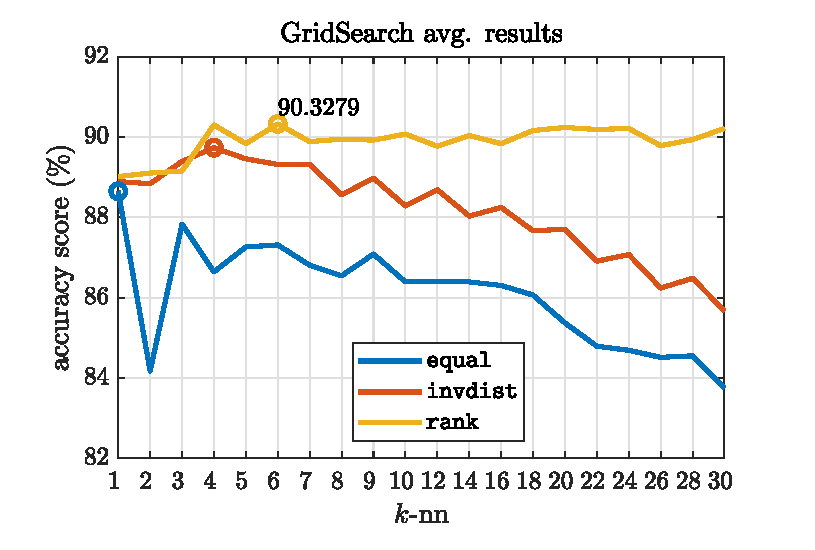
\includegraphics[width=0.45\textwidth]{gridsearch}
	\caption{Grid search averaged results. Circles indicate the highest score achieved by the corresponding \texttt{weighfcn}.}
	\label{fig:gridsearch}
\end{figure}

The [6, \texttt{rank}] hyper-parameter pair yielded the highest average accuracy. Seeing that accuracy performance remains high and constant when using rank-weighting we can say it is a \textit{safe} choice because it downplays the role of $k$ when $k \geq 5$.

Refer to the appendix for a more graphical intuition on how the three different weighting functions work. In the appendix we made use of the t-SNE algorithm to represent the semeion-dataset in a 2-dimensional space and ran our $k$-nn implementation over this reduced dataset.
